\chapter{Spark Shuffle分析}

前面讲解了map端和reduce端对Task的不同处理方式,连接它们的桥梁即为Shuffle模块,shuffle用于打通map任务的输出与reduce任务的输入,map任务计算的中间输出结果按照key值哈希后分配给某一个reduce任务。

shuffle过程数据的传输情况可能非常负责
\begin{enumerate}[\bfseries 1]
	\item 数据量大;
	\item 单个Executor内存不足以放下处理完的数据时需要进行磁盘读写;
	\item 数据传输过程中需要压缩和解压缩;
	\item 跨节点传输时需要通过网络;
\end{enumerate}

正因为这众多的因素,shuffle无疑是调优的重点,理解shuffle的版本历史有助于了解shuffle优化的思路。

Shuffle的类型是在SparkContext初始化时确定的,Spark1.6版本如程序\ref{inputPrg:shuffleManager}所示
\begin{codeInput}{Scala}{ShuffleManager的初始化}{shuffleManager}
 //   指定shuffle的类型
 val shortShuffleMgrNames = Map(
 "hash" -> "org.apache.spark.shuffle.hash.HashShuffleManager",
 "sort" -> "org.apache.spark.shuffle.sort.SortShuffleManager",
 "tungsten-sort" -> "org.apache.spark.shuffle.sort.SortShuffleManager")
 val shuffleMgrName = conf.get("spark.shuffle.manager", "sort")
 val shuffleMgrClass = shortShuffleMgrNames.getOrElse(shuffleMgrName.toLowerCase, shuffleMgrName)
 val shuffleManager = instantiateClass[ShuffleManager](shuffleMgrClass)
\end{codeInput}

可以看出ShuffleManager默认类型为SortShuffleManager。

在Executor上执行ShuffleMapTask时,最终会调用ShuffleMapTask.runTask。核心逻辑如程序\ref{inputPrg:runTaskGetShuffleManager}所示
\begin{codeInput}{Scala}{ShuffleMapTask获取ShuffleWriter}{runTaskGetShuffleManager}
 //从SparkEnv中获取shuffleManager
 val manager = SparkEnv.get.shuffleManager
 //从manager中获取Writer,这里是SortShuffleWriter
 writer = manager.getWriter[Any, Any](dep.shuffleHandle, partitionId, context)
 //调用RDD开始运算,运算结果通过Writer进行持久化,之后将文件所有记录写入并创建索引文件,通过MapStatus告知下游Task
 writer.write(rdd.iterator(partition, context).asInstanceOf[Iterator[_ <: Product2[Any, Any]]])
 writer.stop(success = true).get
\end{codeInput}
\section{Shuffle Writer}
\subsection{Hash Based Shuffle Write}
在Spark1.0以前,由于不要求数据有序,shuffle write 的任务很简单:将数据 partition 好,并持久化。之所以要持久化,一方面是要减少内存存储空间压力,另一方面也是为了 fault-tolerance。

shuffle write 的任务很简单,那么实现也很简单:将 shuffle write 的处理逻辑加入到 ShuffleMapStage(ShuffleMapTask 所在的 stage) 的最后,该 stage 的 final RDD 每输出一个 record 就将其 partition 并持久化。此种类型的Writer工作方式如图\ref{fig:hashShuffleWriter}所示, 从图中可以看出4 个 ShuffleMapTask 要在同一个 worker node 上运行,CPU core 数为 2,可以同时运行两个 task。每个 task 的执行结果(该 stage 的 finalRDD 中某个 partition 包含的 records)被逐一写到本地磁盘上。每个 task 包含 R 个缓冲区,R = reducer 个数(也就是下一个 stage 中 task 的个数),缓冲区被称为 bucket\footnote{其实 bucket 是一个广义的概念,代表 ShuffleMapTask 输出结果经过 partition后要存放的地方,这里为了细化数据存放位置和数据名称,仅仅用 bucket 表示缓冲区。},其大小为spark.shuffle.file.buffer.kb ,默认是 32KB(Spark 1.1 版本以前是 100KB)。
\begin{figure}[H] 
	\centering
	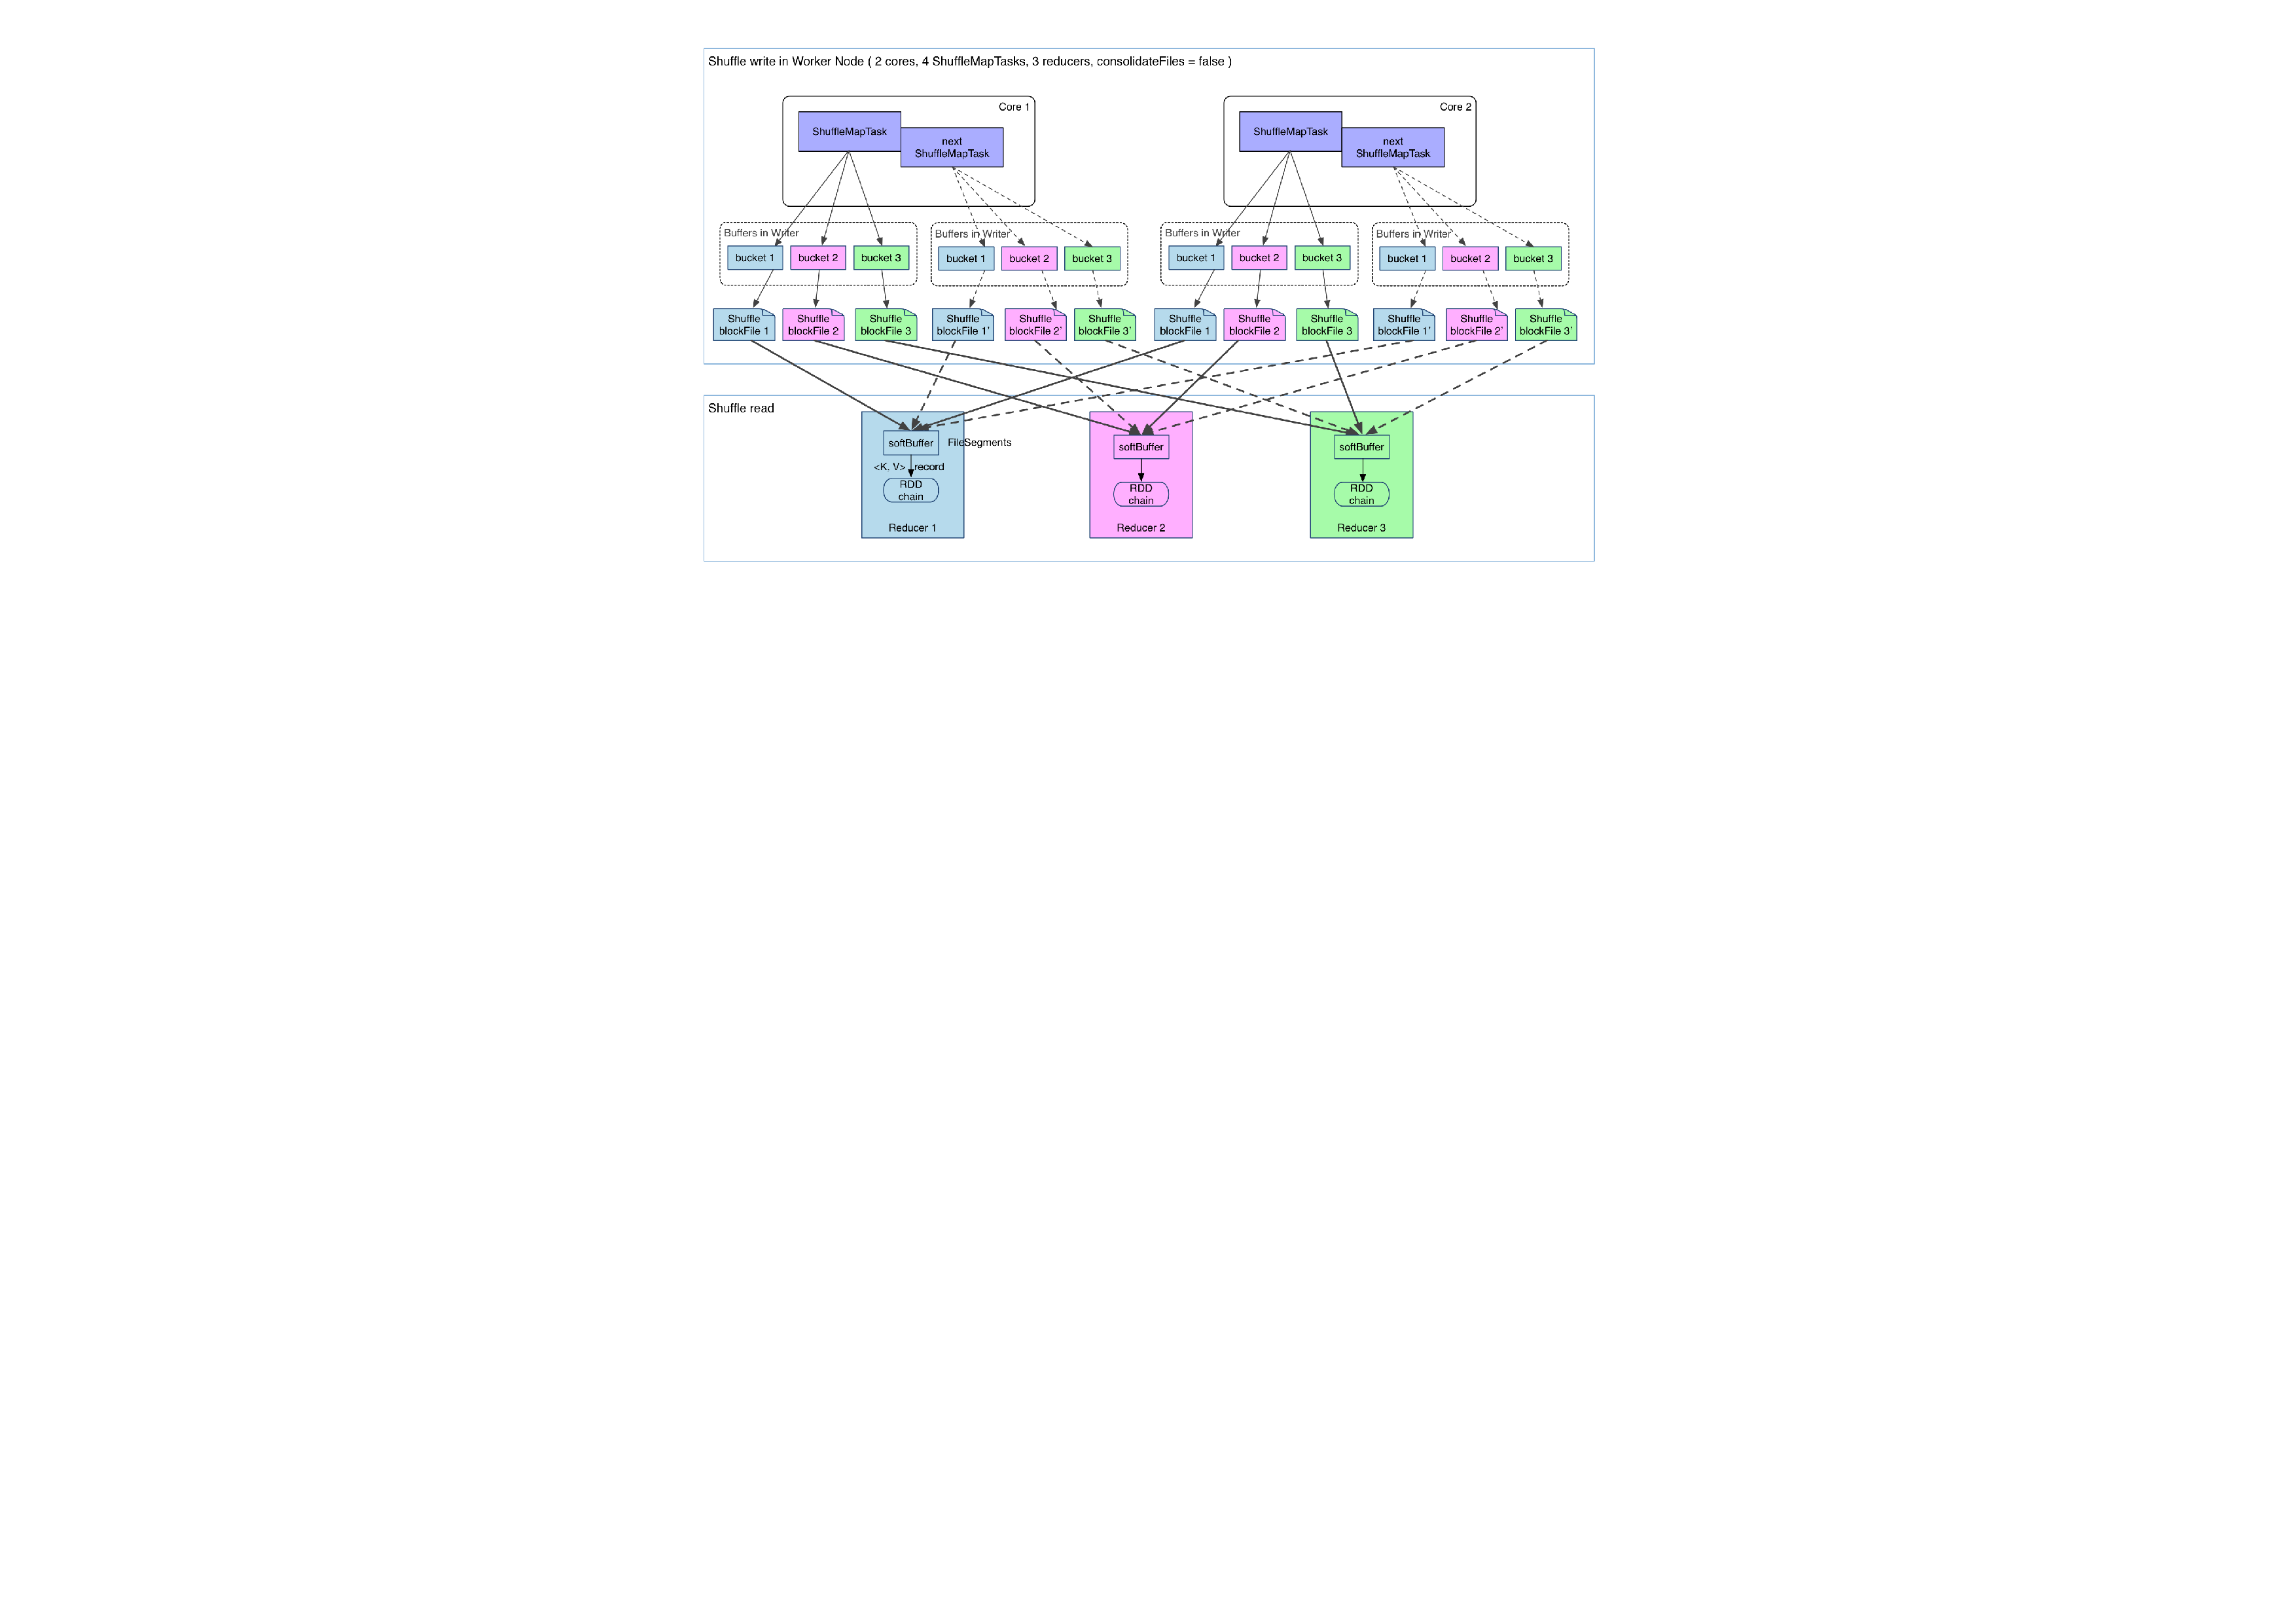
\includegraphics[width=\textwidth]{figures/hashShuffleWriter.pdf}
	\caption{早期的ShuffleWriter工作原理}
	\label{fig:hashShuffleWriter}
\end{figure}
\subsection{Hash Based Shuffle Write存在的问题}

由于ShuffleMapTask需要为每个下游的Task创建一个单独的文件,因此文件的数量就是M*R\footnote{M为shuffleMapTask的数量,R为reduce端Task的数量}个。如果单机28个cpu core,假设节点上20个core用于ShuffleMapTask,R数量为1000个,那么逻辑上会有20000个文件。在实际运行中,Task的数量会更多,这种ShuffleWriter的实现会带来一下问题:
\begin{enumerate}[\bfseries 1]
	\item 缓冲区占用内存空间大
	
	每个节点都可能同时打开多个文件,每次打开文件都会占用一定内存。如上面的20000个文件,每个writer Handler默认需要100KB内存,单个节点就可能达到2GB的内存,当Map端和Reduce同时增加10倍时,整体的内存会更吓人。
	\item 系统随机读增多
	
	当系统存在很多文件比较小但数量比较多的时候,而且机械硬盘在随机读方面的性能特别差,非常容易出现性能瓶颈。
\end{enumerate}
\subsection{Shuffle Consolidate Writer}

为了解决上一小节中Shuffle产生文件较多的问题,之后的Shuffle加入了Consolidate Files机制,它的目标就是减少Shuffle过程文件产生过多的问题,当然第一个问题还是没有解决。它的思想是针对同一个核运行多个ShuffleMapTask的情况下,众多的ShuffleMapTask会将记录写到同一个文件中,下一个会以追加的方式写入而不是新建文件。这样文件数就变为core\footnote{这里指核的数量}*R个文件。此种模式下运行原理如图\ref{fig:consolidate}所示
\begin{figure}[H] 
	\centering
	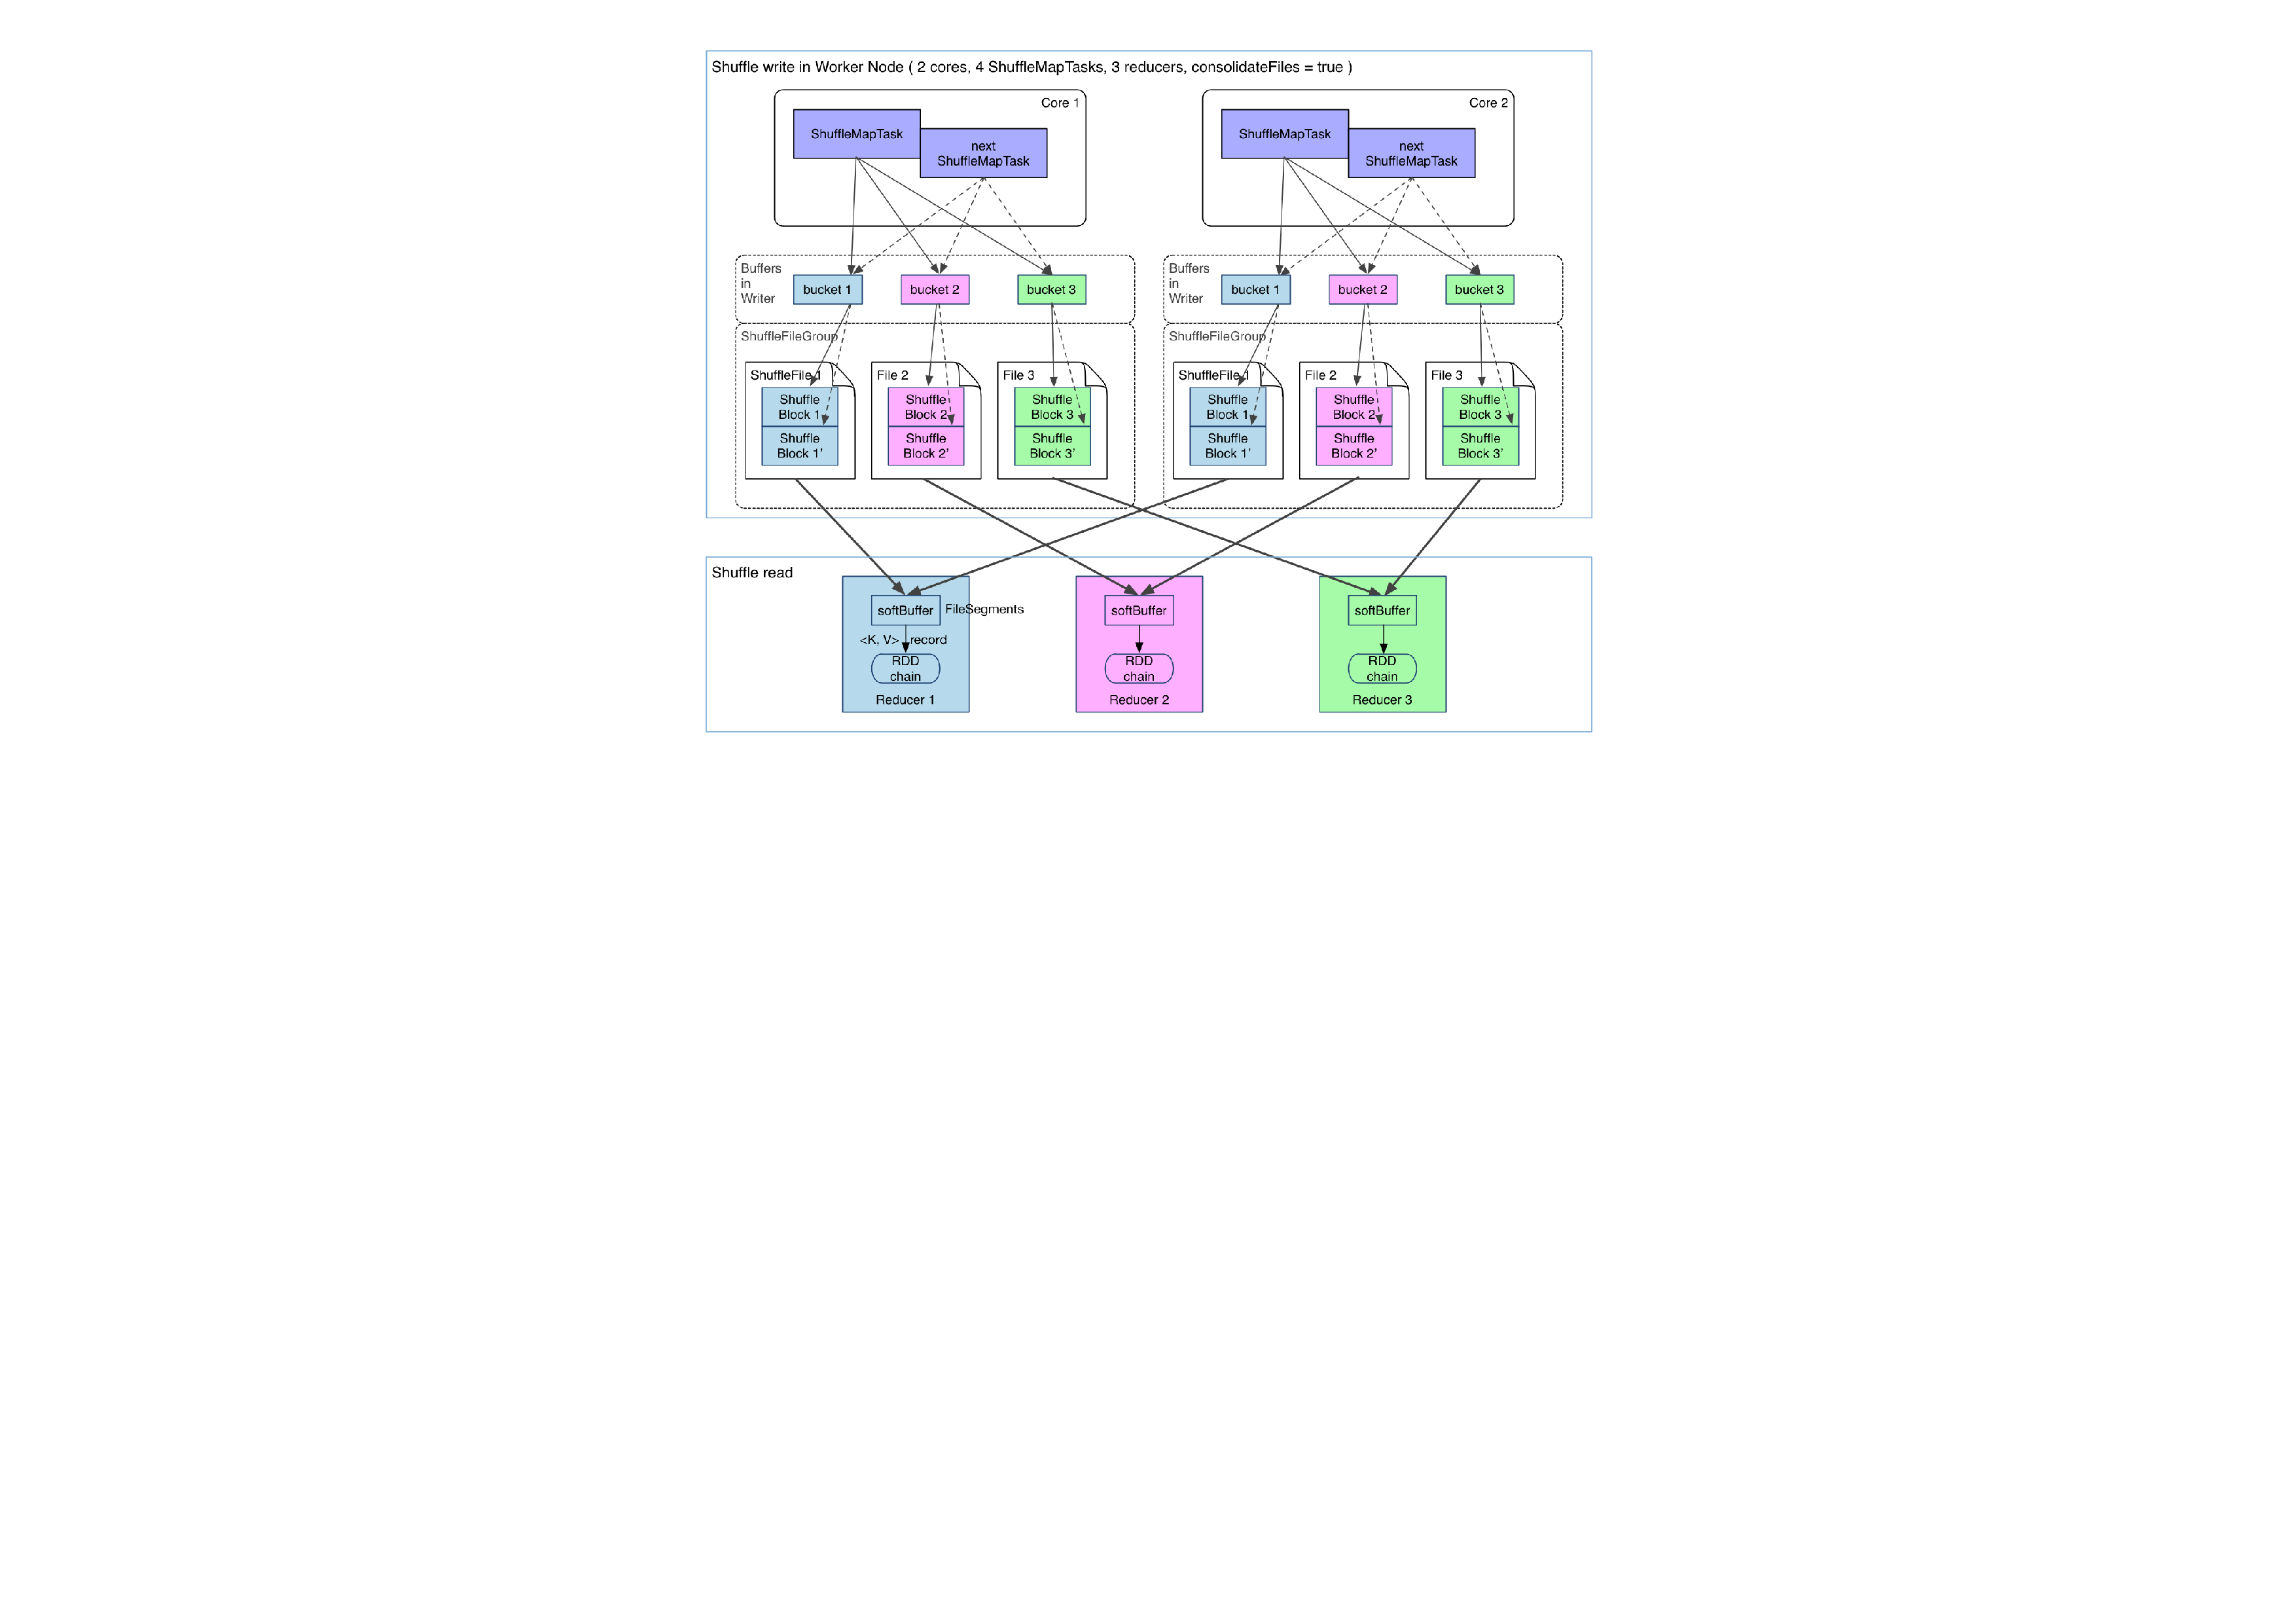
\includegraphics[width=\textwidth]{figures/consolidate.pdf}
	\caption{Shuffle Consolidate Files工作原理}
	\label{fig:consolidate}
\end{figure}

不过这种模式下当每个core只运行一个ShuffleMapTask时,那么就和原来的机制一样了。但是当ShuffleMapTask明显多于core数量时,这种模式下可以显著减少文件的数量。这里还剩下一个问题,下游的Task如何区分文件的不同部分?这部分在后面小节中讲述。

针对Shuffle Consolidate遗留的问题,Spark重新建立了一套Shuffle机制。也就是下面讲述的SortShuffle,这个已经是当前Spark版本的默认选项。
\subsection{Sort Based Write}
此方法的选择是在org.apache.spark.SparkEnv下完成的,本章开头部分已经说明。首先,每个ShuffleMapTask不会为每个Reducer生成一个单独的文件相反,它会将所有的结果写到一个文件里,同时生成一个Index文件,Reducer可以通过这个Index文件取得它需要处理的数据,减少了文件的数量。

Shuffle Map Task 会按照 key 相对应的 partition id 进行排序,对于属于同一个 partition 的 keys 可选的进行或不进行排序。因为对于不需要排序的操作来说,这个排序是有损性能的。对于那些需要 Sort 的操作,比如 sortByKey,这个排序是由 Reducer 完成的。Sort Base Shuffle原理如图\ref{fig:sortshuffle}所示
\begin{figure}[H] 
	\centering
	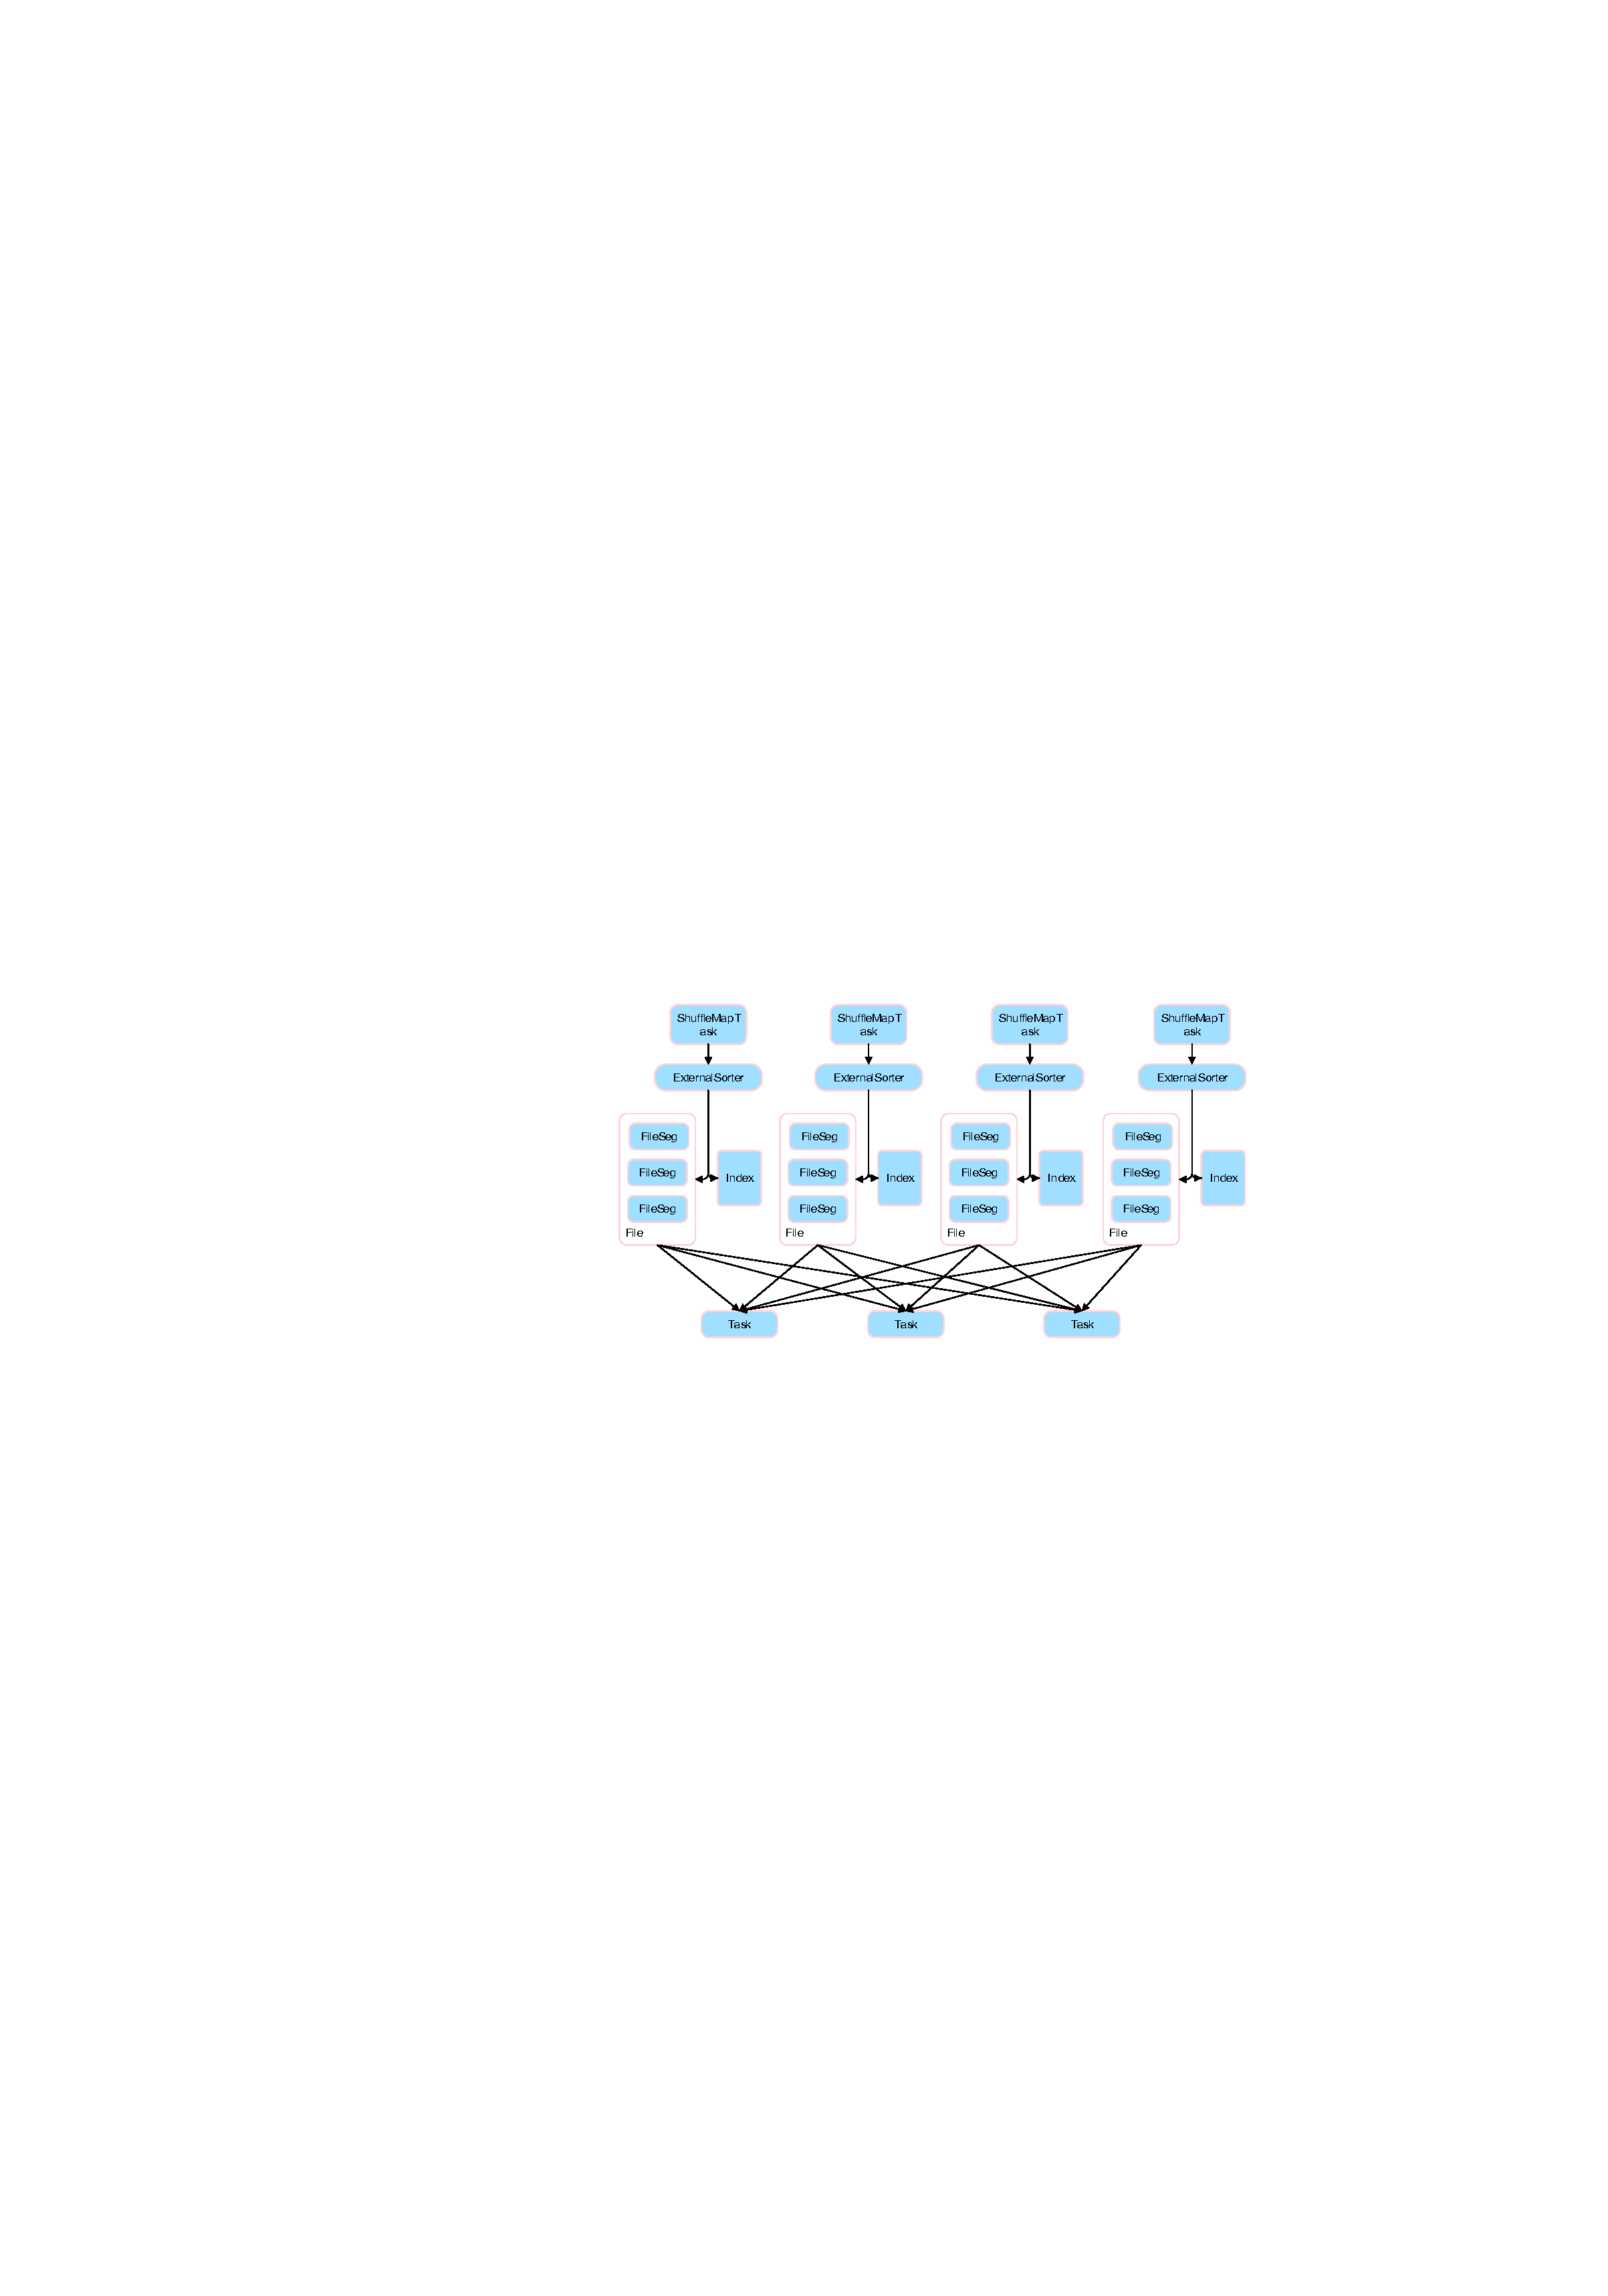
\includegraphics[width=\textwidth]{figures/sortshuffle.pdf}
	\caption{Sort Base Shuffle工作原理}
	\label{fig:sortshuffle}
\end{figure}

为了下游Task获取到其所需要的分区,生成文件的同时会附加Index文件,来记录不同分区的位置信息。
\section{Shuffle Read}

在Stage的边界,要计算ShuffledRDD中的数据,必须先把 MapPartitionsRDD 中的数据 fetch 过来。而下边界,要么将文件写入本地文件系统,以供子Stage读取,要么是最后一个Stage,输出结果。

下游Stage的第一个RDD即为ShuffledRDD,其compute方法中会调用shuffleManager.getReader来读取上游的分区。全部 ShuffleMapTasks 执行完再去 fetch。因为 fetch 来的 FileSegments 要先在内存做缓冲,所以一次 fetch 的 FileSegments 总大小不能太大。Spark 规定这个缓冲界限不能超过 spark.reducer.maxMbInFlight,这里用 softBuffer 表示,默认大小为 48MB。核心的read实现如程序\ref{inputPrg:shuffleReader}所示
\begin{codeInput}{Scala}{Shuffle Read的实现}{shuffleReader}
override def read(): Iterator[Product2[K, C]] = {
val blockFetcherItr = new ShuffleBlockFetcherIterator(context,blockManager.shuffleClient,
blockManager,mapOutputTracker.getMapSizesByExecutorId(handle.shuffleId, startPartition, endPartition),
  SparkEnv.get.conf.getSizeAsMb("spark.reducer.maxSizeInFlight", "48m") * 1024 * 1024)
  ......
  //获取序列化器
  val ser = Serializer.getSerializer(dep.serializer)
  ......
  val interruptibleIter = new InterruptibleIterator[(Any, Any)](context, metricIter)	
  val aggregatedIter: Iterator[Product2[K, C]] = if (dep.aggregator.isDefined) {//需要聚合
    if (dep.mapSideCombine) {//需要map端聚合
      val combinedKeyValuesIterator = interruptibleIter.asInstanceOf[Iterator[(K, C)]]
      dep.aggregator.get.combineCombinersByKey(
      combinedKeyValuesIterator, context)
    } else {//只需在reduce端聚合
      val keyValuesIterator = interruptibleIter.asInstanceOf[Iterator[(K, Nothing)]]
      dep.aggregator.get.combineValuesByKey(keyValuesIterator, context)
    }
  } else {//不需要聚合
    interruptibleIter.asInstanceOf[Iterator[Product2[K, C]]]
  }
  dep.keyOrdering match {//判断是否需要排序
    case Some(keyOrd: Ordering[K]) =>
    //对于需要排序的情况使用ExternalSorter进行排序,注意如果spark.shuffle.spill是false,那么数据不会写到磁盘
      val sorter =new ExternalSorter[K, C, C](context, ordering = Some(keyOrd), serializer = Some(ser))
      sorter.insertAll(aggregatedIter)
      ......
      CompletionIterator[Product2[K, C], Iterator[Product2[K, C]]](sorter.iterator, sorter.stop())
    case None =>aggregatedIter
    //无需排序
  }
}
\end{codeInput}

一个 ShuffleMapStage 形成后,会将该 stage 最后一个 final RDD 注册到 MapOutputTrackerMaster.registerShuffle(shuffleId, rdd.partitions.size),这一步很重要,因为 shuffle 过程需要 MapOutputTrackerMaster 来指示 ShuffleMapTask 输出数据的位置”。因此,reducer 在 shuffle 的时候是要去 driver 里面的 MapOutputTrackerMaster 询问ShuffleMapTask输出的数据位置的,它会调用MapOutputTracke.getStatuses来获得数据的meta数据信息,获得meta数据信息后,它会将这些数据存入Seq[(BlockManagerId, Seq[(BlockId, Long)])]中,然后调用ShuffleBlockFetcherIterator最终发起请求。

\subsection{reduce端读取中间计算结果}
ShuffleBlockFetcherIterator会调用splitLocalRemoteBlocks来划分数据的读取方式,主要是本地数据和远程节点数据。这里Spark限制每次最多启动5个线程到最多5个节点上读取数据,同时通过spark.reducer.maxMbInFlight来适应网络带宽。该部分具体情况如程序\ref{inputPrg:spiltLocalRemoteBlocks}所示
\begin{codeInput}{Scala}{reduce读取数据策略划分}{spiltLocalRemoteBlocks}
private[this] def splitLocalRemoteBlocks():ArrayBuffer[FetchRequest]={
  val targetRequestSize = math.max(maxBytesInFlight / 5, 1L)
  val remoteRequests = new ArrayBuffer[FetchRequest]
  var totalBlocks = 0
  for ((address, blockInfos) <- blocksByAddress) {
    totalBlocks += blockInfos.size
    if (address.executorId == blockManager.blockManagerId.executorId) {//本地获取 local
    //Block在本地,需要过滤大小为0的Block
    localBlocks ++= blockInfos.filter(_._2 != 0).map(_._1)
    numBlocksToFetch += localBlocks.size
    } else {//远程获取 remote
      val iterator = blockInfos.iterator
      var curRequestSize = 0L
      var curBlocks = new ArrayBuffer[(BlockId, Long)]
      while (iterator.hasNext) {//blockId是ShuffleBlockId
        val (blockId, size) = iterator.next()
        if (size > 0) {
          curBlocks += ((blockId, size));remoteBlocks += blockId
          numBlocksToFetch += 1;curRequestSize += size
        } else if (size < 0) {
          throw new BlockException(blockId, "block size " + size)
        }
        if (curRequestSize >= targetRequestSize) {
          //当前总的Size已经可以批量放入一次Request中
          remoteRequests += new FetchRequest(address, curBlocks)
          curBlocks = new ArrayBuffer[(BlockId, Long)]
          curRequestSize = 0
        }
      }
      if (curBlocks.nonEmpty) {//剩余的请求组成一次Request
        remoteRequests += new FetchRequest(address, curBlocks)
      }
    }
  }
  remoteRequests
}
\end{codeInput}
程序\ref{inputPrg:spiltLocalRemoteBlocks}是用于划分哪些Block从本地获取,哪些需要远程拉取,是获取中间计算结果的关键。程序中下列变量比较重要
\begin{enumerate}[\bfseries 1]
	\item targetRequestSize每个远程请求块的最大尺寸
	\item totalblock统计Block总数
	\item localBlocks:ArrayBuffer[BlockId],缓存本地获取的Block的BlockId序列
	\item remoteBlocks:HashSet[BlockId],缓存远程获取的Block的BlockId序列
	\item curBlocks:ArrayBuffer[(BlockId, Long)],远程获取的累加缓存,用于保证每个远程请求的尺寸不超过targetRequestSize。
	\item  curRequestSize当前curBlocks中的所有Block的大小之和,用于保证每个远程请求尺寸不超过targetRequestSize
	\item remoteRequests:ArrayBuffer[FetchRequest],缓存需要远程请求的FetchRequest对象
	\item numBlocksToFetch,一共要获取的Block数量
	\item maxBytesInFlight,单次航班请求的最大字节数。这批请求的总字节数不能超过maxBytesInFlight,并且每一个请求的字节数不能超过maxBytesInFlight的五分之一。
\end{enumerate}
\subsection{本地数据的获取}
上一小节中已经将本地数据块放入localBlocks,对于本地块中的数据将通过fetchLocalBlocks进行获取。具体过程如程序\ref{inputPrg:getLocalBlocks}所示
\begin{codeInput}{Scala}{获取本地块}{getLocalBlocks}
val iter = localBlocks.iterator
while (iter.hasNext) {
  val blockId = iter.next()
  try {
    val buf = blockManager.getBlockData(blockId)
    shuffleMetrics.incLocalBlocksFetched(1)
    shuffleMetrics.incLocalBytesRead(buf.size)
    buf.retain()
    results.put(new SuccessFetchResult(blockId, blockManager.blockManagerId, 0, buf))
  } catch {
  }
}
\end{codeInput}
这里调用了BlockManager.getBlockData获取数据,对于shuffle数据其会调用对应的ShuffleManager.shuffleBlockResolver.getBlockData方法获取数据,其实现如程序\ref{inputPrg:sortShuffleGetBlockData}所示
\begin{codeInput}{Scala}{SortShuffleManager读取shuffle数据实现}{sortShuffleGetBlockData}
//根据ShuffleId和MapId获得索引文件
val indexFile = getIndexFile(blockId.shuffleId, blockId.mapId)
val in = new DataInputStream(new FileInputStream(indexFile))
try {
  ByteStreams.skipFully(in,blockId.reduceId*8)//本次Block的数据区
  val offset = in.readLong()//开始
  val nextOffset = in.readLong()//结束
  new FileSegmentManagedBuffer(transportConf,getDataFile(
  blockId.shuffleId, blockId.mapId),offset,nextOffset - offset)
} 
\end{codeInput}

可以看出它是根据索引文件来获得数据块在数据文件中的具体位置信息的。
\subsection{远程数据的获取}
splitLocalRemoteBlocks返回值为远程数据块,ShuffleBlockFetcherIterator.fetchUpToMaxBytes来发送远程获取请求。通过sendRequest发送读取Block的请求,其中包含中两个回调函数,分别对应着请求成功和请求失败,具体如程序\ref{inputPrg:fetchRemoteBlocks}所示
\begin{codeInput}{Scala}{向远程节点发送读取Block请求}{fetchRemoteBlocks}
shuffleClient.fetchBlocks(address.host, address.port, address.executorId, blockIds.toArray,
new BlockFetchingListener {
  override def onBlockFetchSuccess(blockId: String, buf: ManagedBuffer): Unit = {//请求成功
    if (!isZombie) {
      buf.retain()
      results.put(new SuccessFetchResult(BlockId(blockId), address, sizeMap(blockId), buf))
    }
  }	
  override def onBlockFetchFailure(blockId: String, e: Throwable): Unit = {
    results.put(new FailureFetchResult(BlockId(blockId), address, e))
  }
})
\end{codeInput}

程序中的shuffleClient就是blockTransferService,如程序\ref{inputPrg:shuffleClient}所示
\begin{codeInput}{Scala}{BlockManager获取shuffleClient}{shuffleClient}
val externalShuffleServiceEnabled = conf.getBoolean("spark.shuffle.service.enabled", false)
//externalShuffleServiceEnabled默认为false
private[spark] val shuffleClient = if (externalShuffleServiceEnabled) {
  val transConf = SparkTransportConf.fromSparkConf(conf, "shuffle", numUsableCores)
  new ExternalShuffleClient(transConf, securityManager, securityManager.isAuthenticationEnabled(),
  securityManager.isSaslEncryptionEnabled())
} else {
  blockTransferService
}
//此部分在SparkEnv里定义,直接通过netty的方式
val blockTransferService = new NettyBlockTransferService(conf, securityManager, numUsableCores)
\end{codeInput}
\subsection{Shuffle Read流程图}
整个shuffle read的执行过程如图\ref{fig:shuffleread}所示
\begin{figure}[H] 
	\centering
	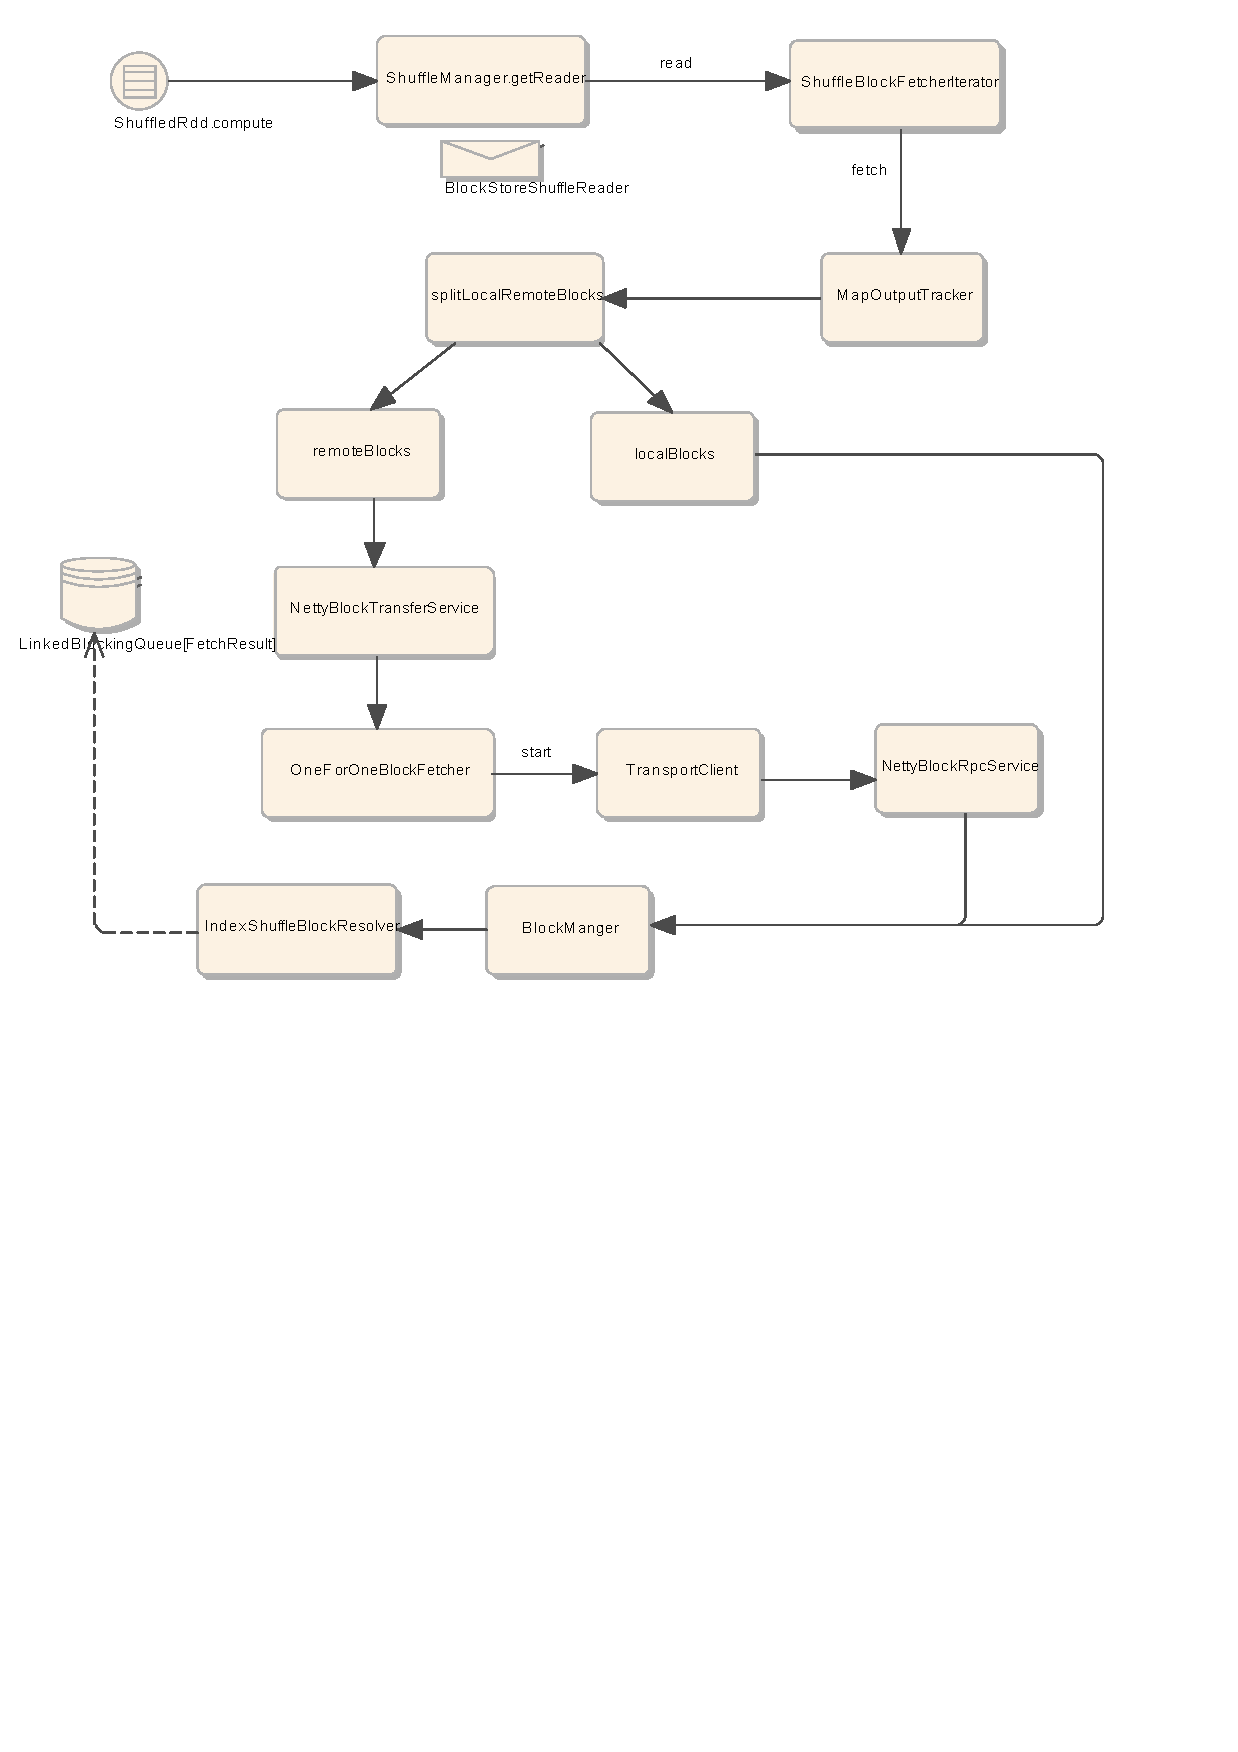
\includegraphics[width=\textwidth]{figures/shuffleRead.pdf}
	\caption{shuffleread详细实现}
	\label{fig:shuffleread}
\end{figure}